\documentclass[]{article}
\usepackage{lmodern}
\usepackage{amssymb,amsmath}
\usepackage{ifxetex,ifluatex}
\usepackage{fixltx2e} % provides \textsubscript
\ifnum 0\ifxetex 1\fi\ifluatex 1\fi=0 % if pdftex
  \usepackage[T1]{fontenc}
  \usepackage[utf8]{inputenc}
\else % if luatex or xelatex
  \ifxetex
    \usepackage{mathspec}
  \else
    \usepackage{fontspec}
  \fi
  \defaultfontfeatures{Ligatures=TeX,Scale=MatchLowercase}
\fi
% use upquote if available, for straight quotes in verbatim environments
\IfFileExists{upquote.sty}{\usepackage{upquote}}{}
% use microtype if available
\IfFileExists{microtype.sty}{%
\usepackage{microtype}
\UseMicrotypeSet[protrusion]{basicmath} % disable protrusion for tt fonts
}{}
\usepackage[margin=1in]{geometry}
\usepackage{hyperref}
\hypersetup{unicode=true,
            pdftitle={Charactersing effect of anaemia on mortality in severe malaria},
            pdfborder={0 0 0},
            breaklinks=true}
\urlstyle{same}  % don't use monospace font for urls
\usepackage{color}
\usepackage{fancyvrb}
\newcommand{\VerbBar}{|}
\newcommand{\VERB}{\Verb[commandchars=\\\{\}]}
\DefineVerbatimEnvironment{Highlighting}{Verbatim}{commandchars=\\\{\}}
% Add ',fontsize=\small' for more characters per line
\usepackage{framed}
\definecolor{shadecolor}{RGB}{248,248,248}
\newenvironment{Shaded}{\begin{snugshade}}{\end{snugshade}}
\newcommand{\KeywordTok}[1]{\textcolor[rgb]{0.13,0.29,0.53}{\textbf{#1}}}
\newcommand{\DataTypeTok}[1]{\textcolor[rgb]{0.13,0.29,0.53}{#1}}
\newcommand{\DecValTok}[1]{\textcolor[rgb]{0.00,0.00,0.81}{#1}}
\newcommand{\BaseNTok}[1]{\textcolor[rgb]{0.00,0.00,0.81}{#1}}
\newcommand{\FloatTok}[1]{\textcolor[rgb]{0.00,0.00,0.81}{#1}}
\newcommand{\ConstantTok}[1]{\textcolor[rgb]{0.00,0.00,0.00}{#1}}
\newcommand{\CharTok}[1]{\textcolor[rgb]{0.31,0.60,0.02}{#1}}
\newcommand{\SpecialCharTok}[1]{\textcolor[rgb]{0.00,0.00,0.00}{#1}}
\newcommand{\StringTok}[1]{\textcolor[rgb]{0.31,0.60,0.02}{#1}}
\newcommand{\VerbatimStringTok}[1]{\textcolor[rgb]{0.31,0.60,0.02}{#1}}
\newcommand{\SpecialStringTok}[1]{\textcolor[rgb]{0.31,0.60,0.02}{#1}}
\newcommand{\ImportTok}[1]{#1}
\newcommand{\CommentTok}[1]{\textcolor[rgb]{0.56,0.35,0.01}{\textit{#1}}}
\newcommand{\DocumentationTok}[1]{\textcolor[rgb]{0.56,0.35,0.01}{\textbf{\textit{#1}}}}
\newcommand{\AnnotationTok}[1]{\textcolor[rgb]{0.56,0.35,0.01}{\textbf{\textit{#1}}}}
\newcommand{\CommentVarTok}[1]{\textcolor[rgb]{0.56,0.35,0.01}{\textbf{\textit{#1}}}}
\newcommand{\OtherTok}[1]{\textcolor[rgb]{0.56,0.35,0.01}{#1}}
\newcommand{\FunctionTok}[1]{\textcolor[rgb]{0.00,0.00,0.00}{#1}}
\newcommand{\VariableTok}[1]{\textcolor[rgb]{0.00,0.00,0.00}{#1}}
\newcommand{\ControlFlowTok}[1]{\textcolor[rgb]{0.13,0.29,0.53}{\textbf{#1}}}
\newcommand{\OperatorTok}[1]{\textcolor[rgb]{0.81,0.36,0.00}{\textbf{#1}}}
\newcommand{\BuiltInTok}[1]{#1}
\newcommand{\ExtensionTok}[1]{#1}
\newcommand{\PreprocessorTok}[1]{\textcolor[rgb]{0.56,0.35,0.01}{\textit{#1}}}
\newcommand{\AttributeTok}[1]{\textcolor[rgb]{0.77,0.63,0.00}{#1}}
\newcommand{\RegionMarkerTok}[1]{#1}
\newcommand{\InformationTok}[1]{\textcolor[rgb]{0.56,0.35,0.01}{\textbf{\textit{#1}}}}
\newcommand{\WarningTok}[1]{\textcolor[rgb]{0.56,0.35,0.01}{\textbf{\textit{#1}}}}
\newcommand{\AlertTok}[1]{\textcolor[rgb]{0.94,0.16,0.16}{#1}}
\newcommand{\ErrorTok}[1]{\textcolor[rgb]{0.64,0.00,0.00}{\textbf{#1}}}
\newcommand{\NormalTok}[1]{#1}
\usepackage{graphicx,grffile}
\makeatletter
\def\maxwidth{\ifdim\Gin@nat@width>\linewidth\linewidth\else\Gin@nat@width\fi}
\def\maxheight{\ifdim\Gin@nat@height>\textheight\textheight\else\Gin@nat@height\fi}
\makeatother
% Scale images if necessary, so that they will not overflow the page
% margins by default, and it is still possible to overwrite the defaults
% using explicit options in \includegraphics[width, height, ...]{}
\setkeys{Gin}{width=\maxwidth,height=\maxheight,keepaspectratio}
\IfFileExists{parskip.sty}{%
\usepackage{parskip}
}{% else
\setlength{\parindent}{0pt}
\setlength{\parskip}{6pt plus 2pt minus 1pt}
}
\setlength{\emergencystretch}{3em}  % prevent overfull lines
\providecommand{\tightlist}{%
  \setlength{\itemsep}{0pt}\setlength{\parskip}{0pt}}
\setcounter{secnumdepth}{0}
% Redefines (sub)paragraphs to behave more like sections
\ifx\paragraph\undefined\else
\let\oldparagraph\paragraph
\renewcommand{\paragraph}[1]{\oldparagraph{#1}\mbox{}}
\fi
\ifx\subparagraph\undefined\else
\let\oldsubparagraph\subparagraph
\renewcommand{\subparagraph}[1]{\oldsubparagraph{#1}\mbox{}}
\fi

%%% Use protect on footnotes to avoid problems with footnotes in titles
\let\rmarkdownfootnote\footnote%
\def\footnote{\protect\rmarkdownfootnote}

%%% Change title format to be more compact
\usepackage{titling}

% Create subtitle command for use in maketitle
\newcommand{\subtitle}[1]{
  \posttitle{
    \begin{center}\large#1\end{center}
    }
}

\setlength{\droptitle}{-2em}

  \title{Charactersing effect of anaemia on mortality in severe malaria}
    \pretitle{\vspace{\droptitle}\centering\huge}
  \posttitle{\par}
    \author{}
    \preauthor{}\postauthor{}
    \date{}
    \predate{}\postdate{}
  

\begin{document}
\maketitle

{
\setcounter{tocdepth}{2}
\tableofcontents
}
\section{Background}\label{background}

This looks at the severe malaria legacy dataset from MORU

\section{Imputation of missing
variables}\label{imputation-of-missing-variables}

Quite a lot of the important covariates are missing in the older
studies. We use linear regression to estimate these unknown variables:

\begin{itemize}
\tightlist
\item
  Mising base deficit is imputed using bicarbonate (if available) else
  using respiratory rate
\item
  Missing Blood urea nitrogen is imputed using creatinine
\end{itemize}

Impute base deficit from bicarbonate

\begin{Shaded}
\begin{Highlighting}[]
\NormalTok{BD_and_bicarbonate =}\StringTok{ }\OperatorTok{!}\KeywordTok{is.na}\NormalTok{(Leg_data}\OperatorTok{$}\NormalTok{BD) }\OperatorTok{&}\StringTok{ }\OperatorTok{!}\KeywordTok{is.na}\NormalTok{(Leg_data}\OperatorTok{$}\NormalTok{bicarbonate)}
\KeywordTok{print}\NormalTok{(}\KeywordTok{paste}\NormalTok{(}\StringTok{'We have '}\NormalTok{, }\KeywordTok{sum}\NormalTok{(BD_and_bicarbonate), }\StringTok{'observations for both bicarbonate and base deficit'}\NormalTok{))}
\end{Highlighting}
\end{Shaded}

\begin{verbatim}
## [1] "We have  5067 observations for both bicarbonate and base deficit"
\end{verbatim}

\begin{Shaded}
\begin{Highlighting}[]
\NormalTok{mod_impute1 =}\StringTok{ }\KeywordTok{lmer}\NormalTok{(BD }\OperatorTok{~}\StringTok{ }\NormalTok{bicarbonate }\OperatorTok{+}\StringTok{ }\NormalTok{(}\DecValTok{1} \OperatorTok{|}\StringTok{ }\NormalTok{studyID) }\OperatorTok{+}\StringTok{ }\NormalTok{(}\DecValTok{1} \OperatorTok{|}\StringTok{ }\NormalTok{country), }\DataTypeTok{data=}\NormalTok{ Leg_data[BD_and_bicarbonate,])}
\NormalTok{missing_BD =}\StringTok{ }\KeywordTok{is.na}\NormalTok{(Leg_data}\OperatorTok{$}\NormalTok{BD)}
\NormalTok{Available_Bicarbonate =}\StringTok{ }\OperatorTok{!}\KeywordTok{is.na}\NormalTok{(Leg_data}\OperatorTok{$}\NormalTok{bicarbonate)}
\KeywordTok{print}\NormalTok{(}\KeywordTok{paste}\NormalTok{(}\KeywordTok{sum}\NormalTok{(missing_BD }\OperatorTok{&}\StringTok{ }\NormalTok{Available_Bicarbonate), }\StringTok{'observations will now be imputed'}\NormalTok{))}
\end{Highlighting}
\end{Shaded}

\begin{verbatim}
## [1] "309 observations will now be imputed"
\end{verbatim}

\begin{Shaded}
\begin{Highlighting}[]
\CommentTok{# impute with model}
\NormalTok{Leg_data}\OperatorTok{$}\NormalTok{BD[missing_BD }\OperatorTok{&}\StringTok{ }\NormalTok{Available_Bicarbonate] =}\StringTok{ }\KeywordTok{predict}\NormalTok{(mod_impute1,}\DataTypeTok{newdata=}\NormalTok{Leg_data[missing_BD }\OperatorTok{&}\StringTok{ }\NormalTok{Available_Bicarbonate,], }\DataTypeTok{re.form=}\OtherTok{NA}\NormalTok{)}
\end{Highlighting}
\end{Shaded}

Impute base deficit from lactate

\begin{Shaded}
\begin{Highlighting}[]
\NormalTok{BD_and_lactate =}\StringTok{ }\OperatorTok{!}\KeywordTok{is.na}\NormalTok{(Leg_data}\OperatorTok{$}\NormalTok{BD) }\OperatorTok{&}\StringTok{ }\OperatorTok{!}\KeywordTok{is.na}\NormalTok{(Leg_data}\OperatorTok{$}\NormalTok{lactate)}
\KeywordTok{print}\NormalTok{(}\KeywordTok{paste}\NormalTok{(}\StringTok{'We have '}\NormalTok{, }\KeywordTok{sum}\NormalTok{(BD_and_lactate), }\StringTok{'observations for both lactate and base deficit'}\NormalTok{))}
\end{Highlighting}
\end{Shaded}

\begin{verbatim}
## [1] "We have  632 observations for both lactate and base deficit"
\end{verbatim}

\begin{Shaded}
\begin{Highlighting}[]
\ControlFlowTok{if}\NormalTok{(}\KeywordTok{length}\NormalTok{(}\KeywordTok{unique}\NormalTok{(Leg_data}\OperatorTok{$}\NormalTok{studyID[BD_and_lactate]))}\OperatorTok{==}\DecValTok{1}\NormalTok{)\{}
\NormalTok{  mod_impute2 =}\StringTok{ }\KeywordTok{lm}\NormalTok{(BD }\OperatorTok{~}\StringTok{ }\NormalTok{lactate, }\DataTypeTok{data=}\NormalTok{ Leg_data[BD_and_lactate,])}
\NormalTok{\} }\ControlFlowTok{else}\NormalTok{ \{}
\NormalTok{  mod_impute2 =}\StringTok{ }\KeywordTok{lmer}\NormalTok{(BD }\OperatorTok{~}\StringTok{ }\NormalTok{lactate }\OperatorTok{+}\StringTok{ }\NormalTok{(}\DecValTok{1} \OperatorTok{|}\StringTok{ }\NormalTok{studyID), }\DataTypeTok{data=}\NormalTok{ Leg_data[BD_and_lactate,])}
\NormalTok{\}}
\NormalTok{missing_BD =}\StringTok{ }\KeywordTok{is.na}\NormalTok{(Leg_data}\OperatorTok{$}\NormalTok{BD)}
\NormalTok{Available_Lactate =}\StringTok{ }\OperatorTok{!}\KeywordTok{is.na}\NormalTok{(Leg_data}\OperatorTok{$}\NormalTok{lactate)}
\KeywordTok{print}\NormalTok{(}\KeywordTok{paste}\NormalTok{(}\KeywordTok{sum}\NormalTok{(missing_BD }\OperatorTok{&}\StringTok{ }\NormalTok{Available_Lactate), }\StringTok{'observations will now be imputed'}\NormalTok{))}
\end{Highlighting}
\end{Shaded}

\begin{verbatim}
## [1] "722 observations will now be imputed"
\end{verbatim}

\begin{Shaded}
\begin{Highlighting}[]
\CommentTok{# impute with model}
\NormalTok{Leg_data}\OperatorTok{$}\NormalTok{BD[missing_BD }\OperatorTok{&}\StringTok{ }\NormalTok{Available_Lactate] =}\StringTok{ }\KeywordTok{predict}\NormalTok{(mod_impute2,}\DataTypeTok{newdata=}\NormalTok{Leg_data[missing_BD }\OperatorTok{&}\StringTok{ }\NormalTok{Available_Lactate,], }\DataTypeTok{re.form=}\OtherTok{NA}\NormalTok{)}
\end{Highlighting}
\end{Shaded}

Impute base deficit from respiratory rate

\begin{Shaded}
\begin{Highlighting}[]
\NormalTok{BD_and_rr =}\StringTok{ }\OperatorTok{!}\KeywordTok{is.na}\NormalTok{(Leg_data}\OperatorTok{$}\NormalTok{BD) }\OperatorTok{&}\StringTok{ }\OperatorTok{!}\KeywordTok{is.na}\NormalTok{(Leg_data}\OperatorTok{$}\NormalTok{rr)}
\KeywordTok{print}\NormalTok{(}\KeywordTok{paste}\NormalTok{(}\StringTok{'We have '}\NormalTok{, }\KeywordTok{sum}\NormalTok{(BD_and_rr), }\StringTok{'observations for both resp rate and base deficit'}\NormalTok{))}
\end{Highlighting}
\end{Shaded}

\begin{verbatim}
## [1] "We have  7572 observations for both resp rate and base deficit"
\end{verbatim}

\begin{Shaded}
\begin{Highlighting}[]
\NormalTok{mod_impute3 =}\StringTok{ }\KeywordTok{lmer}\NormalTok{(BD }\OperatorTok{~}\StringTok{ }\NormalTok{rr }\OperatorTok{+}\StringTok{ }\NormalTok{(}\DecValTok{1} \OperatorTok{|}\StringTok{ }\NormalTok{studyID), }\DataTypeTok{data=}\NormalTok{ Leg_data[BD_and_rr,])}
\NormalTok{missing_BD =}\StringTok{ }\KeywordTok{is.na}\NormalTok{(Leg_data}\OperatorTok{$}\NormalTok{BD)}
\NormalTok{Available_rr =}\StringTok{ }\OperatorTok{!}\KeywordTok{is.na}\NormalTok{(Leg_data}\OperatorTok{$}\NormalTok{rr)}
\KeywordTok{print}\NormalTok{(}\KeywordTok{paste}\NormalTok{(}\KeywordTok{sum}\NormalTok{(missing_BD }\OperatorTok{&}\StringTok{ }\NormalTok{Available_rr), }\StringTok{'observations will now be imputed'}\NormalTok{))}
\end{Highlighting}
\end{Shaded}

\begin{verbatim}
## [1] "1650 observations will now be imputed"
\end{verbatim}

\begin{Shaded}
\begin{Highlighting}[]
\NormalTok{Leg_data}\OperatorTok{$}\NormalTok{BD[missing_BD }\OperatorTok{&}\StringTok{ }\NormalTok{Available_rr] =}\StringTok{ }\KeywordTok{predict}\NormalTok{(mod_impute3,}\DataTypeTok{newdata=}\NormalTok{Leg_data[missing_BD }\OperatorTok{&}\StringTok{ }\NormalTok{Available_rr,], }\DataTypeTok{re.form=}\OtherTok{NA}\NormalTok{)}
\end{Highlighting}
\end{Shaded}

Impute blood urea nitrogen from creatinine:

\begin{Shaded}
\begin{Highlighting}[]
\NormalTok{BUN_and_cr =}\StringTok{ }\OperatorTok{!}\KeywordTok{is.na}\NormalTok{(Leg_data}\OperatorTok{$}\NormalTok{BUN) }\OperatorTok{&}\StringTok{ }\OperatorTok{!}\KeywordTok{is.na}\NormalTok{(Leg_data}\OperatorTok{$}\NormalTok{creatinine)}
\KeywordTok{print}\NormalTok{(}\KeywordTok{paste}\NormalTok{(}\StringTok{'We have '}\NormalTok{, }\KeywordTok{sum}\NormalTok{(BUN_and_cr), }\StringTok{'observations for both blood urea nitrogen and creatinine'}\NormalTok{))}
\end{Highlighting}
\end{Shaded}

\begin{verbatim}
## [1] "We have  1453 observations for both blood urea nitrogen and creatinine"
\end{verbatim}

\begin{Shaded}
\begin{Highlighting}[]
\NormalTok{mod_impute4 =}\StringTok{ }\KeywordTok{lmer}\NormalTok{(BUN }\OperatorTok{~}\StringTok{ }\NormalTok{creatinine }\OperatorTok{+}\StringTok{ }\NormalTok{(}\DecValTok{1} \OperatorTok{|}\StringTok{ }\NormalTok{studyID), }\DataTypeTok{data=}\NormalTok{ Leg_data[BUN_and_cr,])}
\NormalTok{missing_BUN =}\StringTok{ }\KeywordTok{is.na}\NormalTok{(Leg_data}\OperatorTok{$}\NormalTok{BUN)}
\NormalTok{Available_cr =}\StringTok{ }\OperatorTok{!}\KeywordTok{is.na}\NormalTok{(Leg_data}\OperatorTok{$}\NormalTok{creatinine)}
\KeywordTok{print}\NormalTok{(}\KeywordTok{paste}\NormalTok{(}\KeywordTok{sum}\NormalTok{(missing_BUN }\OperatorTok{&}\StringTok{ }\NormalTok{Available_cr), }\StringTok{'observations will now be imputed'}\NormalTok{))}
\end{Highlighting}
\end{Shaded}

\begin{verbatim}
## [1] "679 observations will now be imputed"
\end{verbatim}

\begin{Shaded}
\begin{Highlighting}[]
\NormalTok{Leg_data}\OperatorTok{$}\NormalTok{BUN[missing_BUN }\OperatorTok{&}\StringTok{ }\NormalTok{Available_cr] =}\StringTok{ }\KeywordTok{predict}\NormalTok{(mod_impute4,}\DataTypeTok{newdata=}\NormalTok{Leg_data[missing_BUN }\OperatorTok{&}\StringTok{ }\NormalTok{Available_cr,], }\DataTypeTok{re.form=}\OtherTok{NA}\NormalTok{)}
\end{Highlighting}
\end{Shaded}

Resulting data we can now use: The contributions of the different
studies:

\begin{Shaded}
\begin{Highlighting}[]
\NormalTok{vars_interest =}\StringTok{ }\KeywordTok{c}\NormalTok{(}\StringTok{'outcome'}\NormalTok{,}\StringTok{'HCT'}\NormalTok{,}\StringTok{'LPAR_pct'}\NormalTok{,}\StringTok{'BD'}\NormalTok{,}\StringTok{'BUN'}\NormalTok{,}\StringTok{'poedema'}\NormalTok{,}
                  \StringTok{'convulsions'}\NormalTok{,}\StringTok{'coma'}\NormalTok{,}\StringTok{'AgeInYear'}\NormalTok{,}\StringTok{'drug_class'}\NormalTok{)}
\NormalTok{complete_cases =}\StringTok{ }\KeywordTok{apply}\NormalTok{(Leg_data[,vars_interest], }\DecValTok{1}\NormalTok{, }\ControlFlowTok{function}\NormalTok{(x) }\KeywordTok{sum}\NormalTok{(}\KeywordTok{is.na}\NormalTok{(x))) }\OperatorTok{==}\StringTok{ }\DecValTok{0}
\NormalTok{Complete_Leg_data =}\StringTok{ }\NormalTok{Leg_data[complete_cases,] }\CommentTok{# for the model fitting}
\NormalTok{Complete_Leg_data}\OperatorTok{$}\NormalTok{studyID =}\StringTok{ }\KeywordTok{as.factor}\NormalTok{(}\KeywordTok{as.character}\NormalTok{(Complete_Leg_data}\OperatorTok{$}\NormalTok{studyID))}
\CommentTok{# Whole dataset}
\KeywordTok{table}\NormalTok{(Leg_data}\OperatorTok{$}\NormalTok{studyID)}
\end{Highlighting}
\end{Shaded}

\begin{verbatim}
## 
##          AAV           AQ     AQGambia      AQUAMAT Core Malaria 
##          370          560          579         5494         1122 
##    SEAQUAMAT 
##         1461
\end{verbatim}

\begin{Shaded}
\begin{Highlighting}[]
\CommentTok{# in the complete dataset (all variables recorded)}
\KeywordTok{table}\NormalTok{(Complete_Leg_data}\OperatorTok{$}\NormalTok{studyID)}
\end{Highlighting}
\end{Shaded}

\begin{verbatim}
## 
##          AAV           AQ     AQGambia      AQUAMAT Core Malaria 
##          214          150          168         3666          657 
##    SEAQUAMAT 
##         1333
\end{verbatim}

\begin{Shaded}
\begin{Highlighting}[]
\NormalTok{Complete_Leg_data}\OperatorTok{$}\NormalTok{drug_AS =}\StringTok{ }\DecValTok{0}
\NormalTok{Complete_Leg_data}\OperatorTok{$}\NormalTok{drug_AS[Complete_Leg_data}\OperatorTok{$}\NormalTok{drug_class}\OperatorTok{==}\StringTok{'artemisinin'}\NormalTok{]=}\DecValTok{1}

\CommentTok{# remove infinite log parasitaemias}
\NormalTok{ind_keep =}\StringTok{ }\OperatorTok{!}\NormalTok{(}\KeywordTok{is.infinite}\NormalTok{(Complete_Leg_data}\OperatorTok{$}\NormalTok{LPAR_pct) }\OperatorTok{|}\StringTok{ }\KeywordTok{is.nan}\NormalTok{(Complete_Leg_data}\OperatorTok{$}\NormalTok{LPAR_pct))}
\NormalTok{Complete_Leg_data =}\StringTok{ }\NormalTok{Complete_Leg_data[ind_keep,]}
\end{Highlighting}
\end{Shaded}

Data summaries

\begin{Shaded}
\begin{Highlighting}[]
\NormalTok{Africa =}\StringTok{ }\KeywordTok{c}\NormalTok{(}\StringTok{'The Gambia'}\NormalTok{,}\StringTok{'Mozambique'}\NormalTok{,}\StringTok{'Ghana'}\NormalTok{,}\StringTok{'Kenya'}\NormalTok{,}\StringTok{'Nigeria'}\NormalTok{,}\StringTok{'Tanzania'}\NormalTok{,}\StringTok{'Uganda'}\NormalTok{,}\StringTok{'Rwanda'}\NormalTok{,}\StringTok{'Congo'}\NormalTok{)}
\NormalTok{Asia =}\StringTok{ }\KeywordTok{c}\NormalTok{(}\StringTok{'Thailand'}\NormalTok{,}\StringTok{'Vietnam'}\NormalTok{,}\StringTok{'Bangladesh'}\NormalTok{,}\StringTok{'Myanmar'}\NormalTok{,}\StringTok{'India'}\NormalTok{,}\StringTok{'Indonesia'}\NormalTok{)}
\KeywordTok{writeLines}\NormalTok{(}\KeywordTok{paste}\NormalTok{(}\StringTok{'Children in Africa:'}\NormalTok{,}
                 \KeywordTok{sum}\NormalTok{(Complete_Leg_data}\OperatorTok{$}\NormalTok{AgeInYear }\OperatorTok{<}\StringTok{ }\DecValTok{15} \OperatorTok{&}\StringTok{ }\NormalTok{Complete_Leg_data}\OperatorTok{$}\NormalTok{country }\OperatorTok\StringTok{ }\NormalTok{Africa)))}
\end{Highlighting}
\end{Shaded}

\begin{verbatim}
## Children in Africa: 3779
\end{verbatim}

\begin{Shaded}
\begin{Highlighting}[]
\KeywordTok{writeLines}\NormalTok{(}\KeywordTok{paste}\NormalTok{(}\StringTok{'Adults in Africa:'}\NormalTok{,}
                 \KeywordTok{sum}\NormalTok{(Complete_Leg_data}\OperatorTok{$}\NormalTok{AgeInYear }\OperatorTok{>=}\StringTok{ }\DecValTok{15} \OperatorTok{&}\StringTok{ }\NormalTok{Complete_Leg_data}\OperatorTok{$}\NormalTok{country }\OperatorTok\StringTok{ }\NormalTok{Africa)))}
\end{Highlighting}
\end{Shaded}

\begin{verbatim}
## Adults in Africa: 44
\end{verbatim}

\begin{Shaded}
\begin{Highlighting}[]
\KeywordTok{writeLines}\NormalTok{(}\KeywordTok{paste}\NormalTok{(}\StringTok{'Children in Asia:'}\NormalTok{,}
                 \KeywordTok{sum}\NormalTok{(Complete_Leg_data}\OperatorTok{$}\NormalTok{AgeInYear }\OperatorTok{<}\StringTok{ }\DecValTok{15} \OperatorTok{&}\StringTok{ }\NormalTok{Complete_Leg_data}\OperatorTok{$}\NormalTok{country }\OperatorTok\StringTok{ }\NormalTok{Asia)))}
\end{Highlighting}
\end{Shaded}

\begin{verbatim}
## Children in Asia: 198
\end{verbatim}

\begin{Shaded}
\begin{Highlighting}[]
\KeywordTok{writeLines}\NormalTok{(}\KeywordTok{paste}\NormalTok{(}\StringTok{'Adults in Asia:'}\NormalTok{,}
                 \KeywordTok{sum}\NormalTok{(Complete_Leg_data}\OperatorTok{$}\NormalTok{AgeInYear }\OperatorTok{>=}\StringTok{ }\DecValTok{15} \OperatorTok{&}\StringTok{ }\NormalTok{Complete_Leg_data}\OperatorTok{$}\NormalTok{country }\OperatorTok\StringTok{ }\NormalTok{Asia)))}
\end{Highlighting}
\end{Shaded}

\begin{verbatim}
## Adults in Asia: 2095
\end{verbatim}

\section{Exploratory analysis}\label{exploratory-analysis}

\begin{Shaded}
\begin{Highlighting}[]
\ControlFlowTok{for}\NormalTok{(s }\ControlFlowTok{in} \KeywordTok{unique}\NormalTok{(Complete_Leg_data}\OperatorTok{$}\NormalTok{studyID))\{}
  \KeywordTok{print}\NormalTok{(}\KeywordTok{paste}\NormalTok{(s, }\StringTok{', mortality of:'}\NormalTok{, }\KeywordTok{round}\NormalTok{(}\DecValTok{100}\OperatorTok{*}\KeywordTok{mean}\NormalTok{(Complete_Leg_data}\OperatorTok{$}\NormalTok{outcome[Complete_Leg_data}\OperatorTok{$}\NormalTok{studyID}\OperatorTok{==}\NormalTok{s])),}\StringTok{'%'}\NormalTok{))}
\NormalTok{\}}
\end{Highlighting}
\end{Shaded}

\begin{verbatim}
## [1] "Core Malaria , mortality of: 23 %"
## [1] "AQGambia , mortality of: 12 %"
## [1] "AAV , mortality of: 12 %"
## [1] "SEAQUAMAT , mortality of: 18 %"
## [1] "AQUAMAT , mortality of: 9 %"
## [1] "AQ , mortality of: 23 %"
\end{verbatim}

\begin{Shaded}
\begin{Highlighting}[]
\ControlFlowTok{for}\NormalTok{(s }\ControlFlowTok{in} \KeywordTok{unique}\NormalTok{(Complete_Leg_data}\OperatorTok{$}\NormalTok{studyID))\{}
  \KeywordTok{print}\NormalTok{(}\KeywordTok{paste0}\NormalTok{(s, }\StringTok{', ages:'}\NormalTok{, }\KeywordTok{round}\NormalTok{(}\KeywordTok{quantile}\NormalTok{(Complete_Leg_data}\OperatorTok{$}\NormalTok{AgeInYear[Complete_Leg_data}\OperatorTok{$}\NormalTok{studyID}\OperatorTok{==}\NormalTok{s], }\DataTypeTok{probs =} \KeywordTok{c}\NormalTok{(}\DecValTok{0}\NormalTok{,.}\DecValTok{5}\NormalTok{,}\DecValTok{1}\NormalTok{))), }\DataTypeTok{collapse =} \StringTok{' '}\NormalTok{))}
\NormalTok{\}}
\end{Highlighting}
\end{Shaded}

\begin{verbatim}
## [1] "Core Malaria, ages:1 Core Malaria, ages:27 Core Malaria, ages:75"
## [1] "AQGambia, ages:1 AQGambia, ages:4 AQGambia, ages:9"
## [1] "AAV, ages:15 AAV, ages:34 AAV, ages:77"
## [1] "SEAQUAMAT, ages:2 SEAQUAMAT, ages:25 SEAQUAMAT, ages:87"
## [1] "AQUAMAT, ages:0 AQUAMAT, ages:2 AQUAMAT, ages:78"
## [1] "AQ, ages:15 AQ, ages:30 AQ, ages:74"
\end{verbatim}

\begin{Shaded}
\begin{Highlighting}[]
\ControlFlowTok{for}\NormalTok{(s }\ControlFlowTok{in} \KeywordTok{unique}\NormalTok{(Complete_Leg_data}\OperatorTok{$}\NormalTok{studyID))\{}
  \KeywordTok{print}\NormalTok{(s)}
  \KeywordTok{print}\NormalTok{(}\KeywordTok{table}\NormalTok{(Complete_Leg_data}\OperatorTok{$}\NormalTok{drug[Complete_Leg_data}\OperatorTok{$}\NormalTok{studyID}\OperatorTok{==}\NormalTok{s]))}
\NormalTok{\}}
\end{Highlighting}
\end{Shaded}

\begin{verbatim}
## [1] "Core Malaria"
## 
##  Amodiaquine   Artemether   Artesunate  Chloroquine Lumefantrine 
##            0           11          368            2            0 
##   Mefloquine          NAC      Quinine 
##            7            6          262 
## [1] "AQGambia"
## 
##  Amodiaquine   Artemether   Artesunate  Chloroquine Lumefantrine 
##            0           82            0            0            0 
##   Mefloquine          NAC      Quinine 
##            0            0           86 
## [1] "AAV"
## 
##  Amodiaquine   Artemether   Artesunate  Chloroquine Lumefantrine 
##            0          102          112            0            0 
##   Mefloquine          NAC      Quinine 
##            0            0            0 
## [1] "SEAQUAMAT"
## 
##  Amodiaquine   Artemether   Artesunate  Chloroquine Lumefantrine 
##            0            0          645            0            0 
##   Mefloquine          NAC      Quinine 
##            0            0          628 
## [1] "AQUAMAT"
## 
##  Amodiaquine   Artemether   Artesunate  Chloroquine Lumefantrine 
##            0            0         1837            0            0 
##   Mefloquine          NAC      Quinine 
##            0            0         1818 
## [1] "AQ"
## 
##  Amodiaquine   Artemether   Artesunate  Chloroquine Lumefantrine 
##            0           73            0            0            0 
##   Mefloquine          NAC      Quinine 
##            0            0           77
\end{verbatim}

Let's look at the key predictive variables. We use a random effects term
to model differences between studies.

\begin{verbatim}
## Linear mixed model fit by REML ['lmerMod']
## Formula: BD ~ HCT + (1 | studyID/country)
##    Data: Complete_Leg_data
## 
## REML criterion at convergence: 40261.9
## 
## Scaled residuals: 
##     Min      1Q  Median      3Q     Max 
## -4.4421 -0.6612 -0.1488  0.5224  4.7209 
## 
## Random effects:
##  Groups          Name        Variance Std.Dev.
##  country:studyID (Intercept)  2.6525  1.6286  
##  studyID         (Intercept)  0.8373  0.9151  
##  Residual                    41.8947  6.4726  
## Number of obs: 6116, groups:  country:studyID, 18; studyID, 6
## 
## Fixed effects:
##              Estimate Std. Error t value
## (Intercept) 10.339058   0.653393   15.82
## HCT         -0.133548   0.009699  -13.77
## 
## Correlation of Fixed Effects:
##     (Intr)
## HCT -0.394
\end{verbatim}

\begin{verbatim}
## Linear mixed model fit by REML ['lmerMod']
## Formula: LPAR_pct ~ HCT + (1 | studyID/country)
##    Data: Complete_Leg_data
## 
## REML criterion at convergence: 13822.9
## 
## Scaled residuals: 
##     Min      1Q  Median      3Q     Max 
## -4.7144 -0.5555  0.1598  0.7265  2.4355 
## 
## Random effects:
##  Groups          Name        Variance Std.Dev.
##  country:studyID (Intercept) 0.00946  0.09726 
##  studyID         (Intercept) 0.07496  0.27379 
##  Residual                    0.55564  0.74541 
## Number of obs: 6116, groups:  country:studyID, 18; studyID, 6
## 
## Fixed effects:
##              Estimate Std. Error t value
## (Intercept)  0.659944   0.121244   5.443
## HCT         -0.004579   0.001116  -4.105
## 
## Correlation of Fixed Effects:
##     (Intr)
## HCT -0.251
\end{verbatim}

\begin{verbatim}
## Linear mixed model fit by REML ['lmerMod']
## Formula: BD ~ log10(BUN) + (1 | studyID/country)
##    Data: Complete_Leg_data
## 
## REML criterion at convergence: 39236.2
## 
## Scaled residuals: 
##     Min      1Q  Median      3Q     Max 
## -5.6063 -0.6369 -0.1041  0.5191  5.0754 
## 
## Random effects:
##  Groups          Name        Variance Std.Dev.
##  country:studyID (Intercept)  2.876   1.696   
##  studyID         (Intercept)  6.858   2.619   
##  Residual                    35.405   5.950   
## Number of obs: 6116, groups:  country:studyID, 18; studyID, 6
## 
## Fixed effects:
##             Estimate Std. Error t value
## (Intercept)  -6.8409     1.2574   -5.44
## log10(BUN)    9.3530     0.2559   36.55
## 
## Correlation of Fixed Effects:
##            (Intr)
## log10(BUN) -0.293
\end{verbatim}

\begin{verbatim}
## Linear mixed model fit by REML ['lmerMod']
## Formula: HCT ~ AgeInYear + (1 | studyID/country)
##    Data: Complete_Leg_data
## 
## REML criterion at convergence: 43534.9
## 
## Scaled residuals: 
##     Min      1Q  Median      3Q     Max 
## -3.1004 -0.7399 -0.0515  0.6927  3.5627 
## 
## Random effects:
##  Groups          Name        Variance Std.Dev.
##  country:studyID (Intercept)  5.722   2.392   
##  studyID         (Intercept)  7.322   2.706   
##  Residual                    71.467   8.454   
## Number of obs: 6116, groups:  country:studyID, 18; studyID, 6
## 
## Fixed effects:
##             Estimate Std. Error t value
## (Intercept) 24.69246    1.36141  18.137
## AgeInYear    0.11159    0.01159   9.626
## 
## Correlation of Fixed Effects:
##           (Intr)
## AgeInYear -0.185
\end{verbatim}

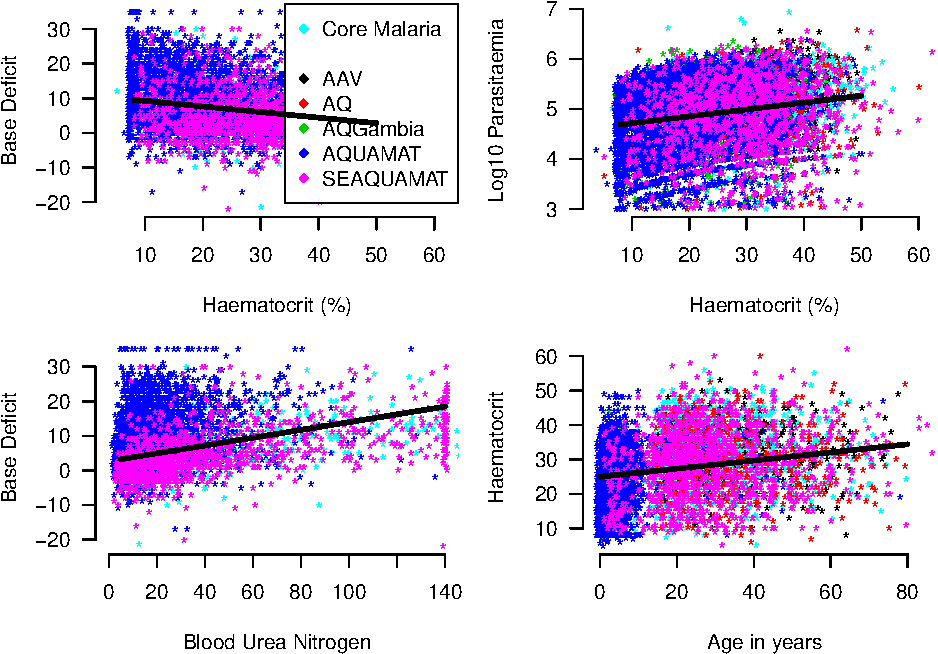
\includegraphics{LegacyAnalysis_files/figure-latex/ExploratoryPlots-1.pdf}

The relationship between haematocrit and death:

\begin{Shaded}
\begin{Highlighting}[]
\KeywordTok{par}\NormalTok{(}\DataTypeTok{las=}\DecValTok{1}\NormalTok{, }\DataTypeTok{bty=}\StringTok{'n'}\NormalTok{)}
\NormalTok{Complete_Leg_data}\OperatorTok{$}\NormalTok{country=}\KeywordTok{as.factor}\NormalTok{(Complete_Leg_data}\OperatorTok{$}\NormalTok{country)}
\NormalTok{modHCT=}\KeywordTok{gam}\NormalTok{(outcome }\OperatorTok{~}\StringTok{ }\KeywordTok{s}\NormalTok{(HCT) }\OperatorTok{+}\StringTok{ }\KeywordTok{s}\NormalTok{(studyID, }\DataTypeTok{bs=}\StringTok{'re'}\NormalTok{) }\OperatorTok{+}\StringTok{ }\KeywordTok{s}\NormalTok{(country, }\DataTypeTok{bs=}\StringTok{'re'}\NormalTok{),}\DataTypeTok{data =}\NormalTok{ Complete_Leg_data, }\DataTypeTok{family=}\StringTok{'binomial'}\NormalTok{)}
\KeywordTok{summary}\NormalTok{(modHCT)}
\end{Highlighting}
\end{Shaded}

\begin{verbatim}
## 
## Family: binomial 
## Link function: logit 
## 
## Formula:
## outcome ~ s(HCT) + s(studyID, bs = "re") + s(country, bs = "re")
## 
## Parametric coefficients:
##             Estimate Std. Error z value Pr(>|z|)    
## (Intercept)  -1.8865     0.2397   -7.87 3.54e-15 ***
## ---
## Signif. codes:  0 '***' 0.001 '**' 0.01 '*' 0.05 '.' 0.1 ' ' 1
## 
## Approximate significance of smooth terms:
##               edf Ref.df  Chi.sq p-value   
## s(HCT)      2.304  2.922   5.482 0.15478   
## s(studyID)  3.611  5.000 314.182 0.00361 **
## s(country) 10.766 14.000 162.027 0.01464 * 
## ---
## Signif. codes:  0 '***' 0.001 '**' 0.01 '*' 0.05 '.' 0.1 ' ' 1
## 
## R-sq.(adj) =  0.0484   Deviance explained = 5.99%
## UBRE = -0.25846  Scale est. = 1         n = 6116
\end{verbatim}

\begin{Shaded}
\begin{Highlighting}[]
\NormalTok{preds =}\StringTok{ }\KeywordTok{predict}\NormalTok{(modHCT, }\DataTypeTok{newdata =} \KeywordTok{data.frame}\NormalTok{(}\DataTypeTok{HCT=}\DecValTok{5}\OperatorTok{:}\DecValTok{45}\NormalTok{, }\DataTypeTok{studyID=}\StringTok{'AQ'}\NormalTok{, }\DataTypeTok{country=}\StringTok{'Thailand'}\NormalTok{, }\DataTypeTok{country=}\DecValTok{1}\NormalTok{), }
                       \DataTypeTok{exclude =} \KeywordTok{c}\NormalTok{(}\StringTok{"s(country)"}\NormalTok{,}\StringTok{"s(studyID)"}\NormalTok{), }\DataTypeTok{type=}\StringTok{'response'}\NormalTok{, }\DataTypeTok{se.fit=}\NormalTok{T)}
\KeywordTok{plot}\NormalTok{(}\DecValTok{5}\OperatorTok{:}\DecValTok{45}\NormalTok{, }\DecValTok{100}\OperatorTok{*}\NormalTok{preds}\OperatorTok{$}\NormalTok{fit, }\DataTypeTok{ylab=}\StringTok{'Probability death (%)'}\NormalTok{, }\DataTypeTok{xlab=}\StringTok{'Haematocrit'}\NormalTok{, }
     \DataTypeTok{type=}\StringTok{'l'}\NormalTok{, }\DataTypeTok{lwd=}\DecValTok{3}\NormalTok{,}\DataTypeTok{ylim =} \KeywordTok{c}\NormalTok{(}\DecValTok{5}\NormalTok{,}\DecValTok{25}\NormalTok{))}
\KeywordTok{lines}\NormalTok{(}\DecValTok{5}\OperatorTok{:}\DecValTok{45}\NormalTok{, }\DecValTok{100}\OperatorTok{*}\NormalTok{preds}\OperatorTok{$}\NormalTok{fit }\OperatorTok{+}\StringTok{ }\DecValTok{100}\OperatorTok{*}\DecValTok{2}\OperatorTok{*}\NormalTok{preds}\OperatorTok{$}\NormalTok{se.fit, }\DataTypeTok{lty=}\DecValTok{2}\NormalTok{,}\DataTypeTok{lwd=}\DecValTok{2}\NormalTok{)}
\KeywordTok{lines}\NormalTok{(}\DecValTok{5}\OperatorTok{:}\DecValTok{45}\NormalTok{, }\DecValTok{100}\OperatorTok{*}\NormalTok{preds}\OperatorTok{$}\NormalTok{fit }\OperatorTok{-}\StringTok{ }\DecValTok{100}\OperatorTok{*}\DecValTok{2}\OperatorTok{*}\NormalTok{preds}\OperatorTok{$}\NormalTok{se.fit,}\DataTypeTok{lty=}\DecValTok{2}\NormalTok{,}\DataTypeTok{lwd=}\DecValTok{2}\NormalTok{)}
\KeywordTok{abline}\NormalTok{(}\DataTypeTok{h =} \KeywordTok{min}\NormalTok{(}\DecValTok{100}\OperatorTok{*}\NormalTok{preds}\OperatorTok{$}\NormalTok{fit), }\DataTypeTok{lwd=}\DecValTok{2}\NormalTok{, }\DataTypeTok{lty=}\DecValTok{3}\NormalTok{)}
\end{Highlighting}
\end{Shaded}

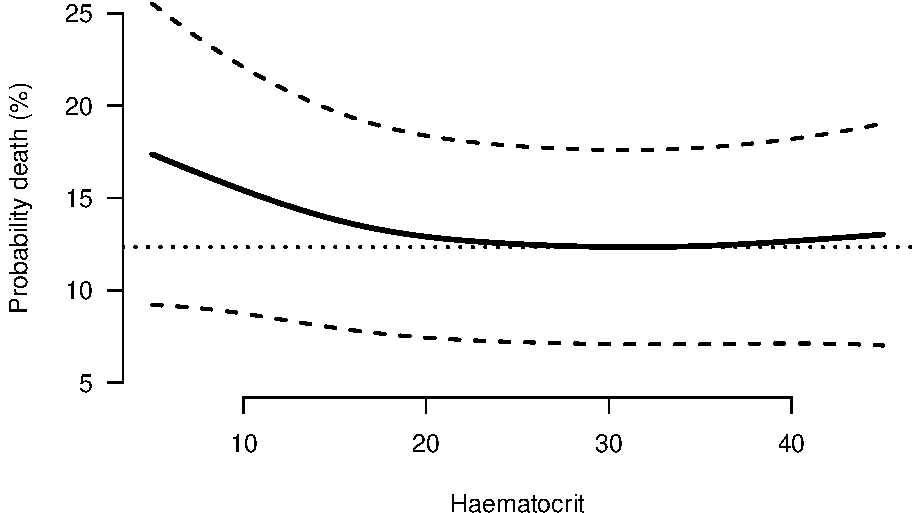
\includegraphics{LegacyAnalysis_files/figure-latex/HCTalone-1.pdf}

\section{Predictive value of anaemia on death adjusting for
confounders}\label{predictive-value-of-anaemia-on-death-adjusting-for-confounders}

Before fitting the more complex GAM models we explore the standard glm
(logistic regression) models.

\begin{Shaded}
\begin{Highlighting}[]
\NormalTok{mod_full_GLM =}\StringTok{ }\KeywordTok{glmer}\NormalTok{(outcome }\OperatorTok{~}\StringTok{ }\NormalTok{HCT }\OperatorTok{+}\StringTok{ }\NormalTok{LPAR_pct }\OperatorTok{+}\StringTok{ }\NormalTok{AgeInYear }\OperatorTok{+}\StringTok{ }\NormalTok{coma }\OperatorTok{+}\StringTok{ }\NormalTok{convulsions }\OperatorTok{+}
\StringTok{                       }\NormalTok{poedema }\OperatorTok{+}\StringTok{ }\KeywordTok{log10}\NormalTok{(BUN) }\OperatorTok{+}\StringTok{ }\NormalTok{BD }\OperatorTok{+}\StringTok{ }\NormalTok{drug_AS }\OperatorTok{+}\StringTok{ }
\StringTok{                       }\NormalTok{(}\DecValTok{1} \OperatorTok{|}\StringTok{ }\NormalTok{studyID) }\OperatorTok{+}\StringTok{ }\NormalTok{(}\DecValTok{1} \OperatorTok{|}\StringTok{ }\NormalTok{country),}
                     \DataTypeTok{data =}\NormalTok{ Complete_Leg_data, }\DataTypeTok{family=}\NormalTok{binomial)}
\end{Highlighting}
\end{Shaded}

\begin{verbatim}
## Warning in checkConv(attr(opt, "derivs"), opt$par, ctrl =
## control$checkConv, : Model failed to converge with max|grad| = 0.00101495
## (tol = 0.001, component 1)
\end{verbatim}

\begin{Shaded}
\begin{Highlighting}[]
\KeywordTok{summary}\NormalTok{(mod_full_GLM)}
\end{Highlighting}
\end{Shaded}

\begin{verbatim}
## Generalized linear mixed model fit by maximum likelihood (Laplace
##   Approximation) [glmerMod]
##  Family: binomial  ( logit )
## Formula: 
## outcome ~ HCT + LPAR_pct + AgeInYear + coma + convulsions + poedema +  
##     log10(BUN) + BD + drug_AS + (1 | studyID) + (1 | country)
##    Data: Complete_Leg_data
## 
##      AIC      BIC   logLik deviance df.resid 
##   3459.7   3540.3  -1717.8   3435.7     6104 
## 
## Scaled residuals: 
##     Min      1Q  Median      3Q     Max 
## -3.9034 -0.3324 -0.1914 -0.1076 15.4072 
## 
## Random effects:
##  Groups  Name        Variance  Std.Dev. 
##  country (Intercept) 1.501e-01 3.875e-01
##  studyID (Intercept) 1.919e-09 4.381e-05
## Number of obs: 6116, groups:  country, 15; studyID, 6
## 
## Fixed effects:
##               Estimate Std. Error z value Pr(>|z|)    
## (Intercept)  -7.000057   0.306929 -22.807  < 2e-16 ***
## HCT           0.016441   0.005284   3.111 0.001863 ** 
## LPAR_pct     -0.001281   0.060471  -0.021 0.983095    
## AgeInYear     0.013715   0.003840   3.571 0.000355 ***
## coma          1.338046   0.100906  13.260  < 2e-16 ***
## convulsions1  0.513532   0.116864   4.394 1.11e-05 ***
## poedema1      0.543720   0.385373   1.411 0.158276    
## log10(BUN)    1.778368   0.166012  10.712  < 2e-16 ***
## BD            0.121719   0.007183  16.944  < 2e-16 ***
## drug_AS      -0.343604   0.090337  -3.804 0.000143 ***
## ---
## Signif. codes:  0 '***' 0.001 '**' 0.01 '*' 0.05 '.' 0.1 ' ' 1
## 
## Correlation of Fixed Effects:
##             (Intr) HCT    LPAR_p AgInYr coma   cnvls1 poedm1 l10(BU BD    
## HCT         -0.483                                                        
## LPAR_pct    -0.041  0.030                                                 
## AgeInYear    0.039 -0.178  0.001                                          
## coma        -0.163 -0.027  0.075  0.000                                   
## convulsins1 -0.133 -0.073  0.017  0.108 -0.220                            
## poedema1    -0.004 -0.005 -0.006 -0.048  0.027  0.000                     
## log10(BUN)  -0.700  0.064 -0.047 -0.245 -0.014  0.103  0.006              
## BD          -0.148  0.199 -0.180  0.135 -0.024  0.024 -0.008 -0.262       
## drug_AS     -0.091 -0.012 -0.024 -0.022  0.007  0.004 -0.025 -0.044 -0.020
## convergence code: 0
## Model failed to converge with max|grad| = 0.00101495 (tol = 0.001, component 1)
\end{verbatim}

Now let's make counterfactual predictions of anaemia on death for the
patients in the database.

\begin{Shaded}
\begin{Highlighting}[]
\NormalTok{myquantiles =}\StringTok{ }\KeywordTok{c}\NormalTok{(}\FloatTok{0.25}\NormalTok{,}\FloatTok{0.5}\NormalTok{,}\FloatTok{0.75}\NormalTok{) }\CommentTok{# this is 50% predictive interval}

\NormalTok{overall_median_mortality =}\StringTok{ }\KeywordTok{median}\NormalTok{(}\DecValTok{100}\OperatorTok{*}\KeywordTok{predict}\NormalTok{(mod_full_GLM, }\DataTypeTok{type=}\StringTok{'response'}\NormalTok{))}
\KeywordTok{par}\NormalTok{(}\DataTypeTok{las=}\DecValTok{1}\NormalTok{, }\DataTypeTok{bty=}\StringTok{'n'}\NormalTok{)}
\NormalTok{x_hcts =}\StringTok{ }\KeywordTok{seq}\NormalTok{(}\DecValTok{4}\NormalTok{,}\DecValTok{45}\NormalTok{, }\DataTypeTok{by=}\DecValTok{1}\NormalTok{)}
\NormalTok{probs_lin =}\StringTok{ }\KeywordTok{array}\NormalTok{(}\DataTypeTok{dim =} \KeywordTok{c}\NormalTok{(}\DecValTok{3}\NormalTok{, }\KeywordTok{length}\NormalTok{(x_hcts)))}
\ControlFlowTok{for}\NormalTok{(i }\ControlFlowTok{in} \DecValTok{1}\OperatorTok{:}\KeywordTok{length}\NormalTok{(x_hcts))\{}
\NormalTok{  mydata =}\StringTok{ }\NormalTok{Complete_Leg_data}
\NormalTok{  mydata}\OperatorTok{$}\NormalTok{HCT=x_hcts[i]}
\NormalTok{  ys =}\StringTok{ }\DecValTok{100}\OperatorTok{*}\KeywordTok{predict}\NormalTok{(mod_full_GLM, }\DataTypeTok{newdata =}\NormalTok{ mydata, }\DataTypeTok{re.form=}\OtherTok{NA}\NormalTok{, }\DataTypeTok{type=}\StringTok{'response'}\NormalTok{)}
\NormalTok{  probs_lin[,i] =}\StringTok{ }\KeywordTok{quantile}\NormalTok{(ys, }\DataTypeTok{probs=}\NormalTok{myquantiles)}
\NormalTok{\}}
\end{Highlighting}
\end{Shaded}

The way to interpret this `counterfactual' plot is as follows: suppose
that every individual in the dataset was assigned (as in a intervention)
a specific haematocrit \(X\), what would the resulting per patient
probability of death be. Here we summarise these probabilities by the
predicted mean probability of death and 80\% predictive intervals.

\begin{Shaded}
\begin{Highlighting}[]
\KeywordTok{plot}\NormalTok{(x_hcts,probs_lin[}\DecValTok{2}\NormalTok{,], }\DataTypeTok{xlim=}\KeywordTok{c}\NormalTok{(}\DecValTok{4}\NormalTok{,}\DecValTok{45}\NormalTok{), }\DataTypeTok{ylab=}\StringTok{'Predicted probability of death'}\NormalTok{, }
     \DataTypeTok{xlab=}\StringTok{'Haematocrit (%)'}\NormalTok{, }\DataTypeTok{ylim=}\KeywordTok{c}\NormalTok{(}\DecValTok{0}\NormalTok{,}\DecValTok{20}\NormalTok{), }\DataTypeTok{lty=}\DecValTok{1}\NormalTok{, }\DataTypeTok{lwd=}\DecValTok{3}\NormalTok{, }\DataTypeTok{type=}\StringTok{'l'}\NormalTok{)}
\KeywordTok{lines}\NormalTok{(x_hcts, probs_lin[}\DecValTok{1}\NormalTok{,], }\DataTypeTok{lty=}\DecValTok{2}\NormalTok{, }\DataTypeTok{lwd=}\DecValTok{2}\NormalTok{)}
\KeywordTok{lines}\NormalTok{(x_hcts, probs_lin[}\DecValTok{3}\NormalTok{,], }\DataTypeTok{lty=}\DecValTok{2}\NormalTok{, }\DataTypeTok{lwd=}\DecValTok{2}\NormalTok{)}
\KeywordTok{abline}\NormalTok{(}\DataTypeTok{h=}\NormalTok{overall_median_mortality, }\DataTypeTok{lwd=}\DecValTok{3}\NormalTok{, }\DataTypeTok{col=}\StringTok{'blue'}\NormalTok{,}\DataTypeTok{lty=}\DecValTok{2}\NormalTok{)}
\KeywordTok{legend}\NormalTok{(}\StringTok{'topleft'}\NormalTok{, }\DataTypeTok{col=}\KeywordTok{c}\NormalTok{(}\StringTok{'black'}\NormalTok{,}\StringTok{'black'}\NormalTok{,}\StringTok{'blue'}\NormalTok{), }\DataTypeTok{lwd=}\DecValTok{3}\NormalTok{, }\DataTypeTok{lty=}\KeywordTok{c}\NormalTok{(}\DecValTok{1}\NormalTok{,}\DecValTok{2}\NormalTok{,}\DecValTok{2}\NormalTok{),}
       \DataTypeTok{legend =} \KeywordTok{c}\NormalTok{(}\StringTok{'Median counterfactual value'}\NormalTok{, }\StringTok{'25th and 75th counterfactual quantiles'}\NormalTok{,}\StringTok{'Retrodicted median value'}\NormalTok{))}
\end{Highlighting}
\end{Shaded}

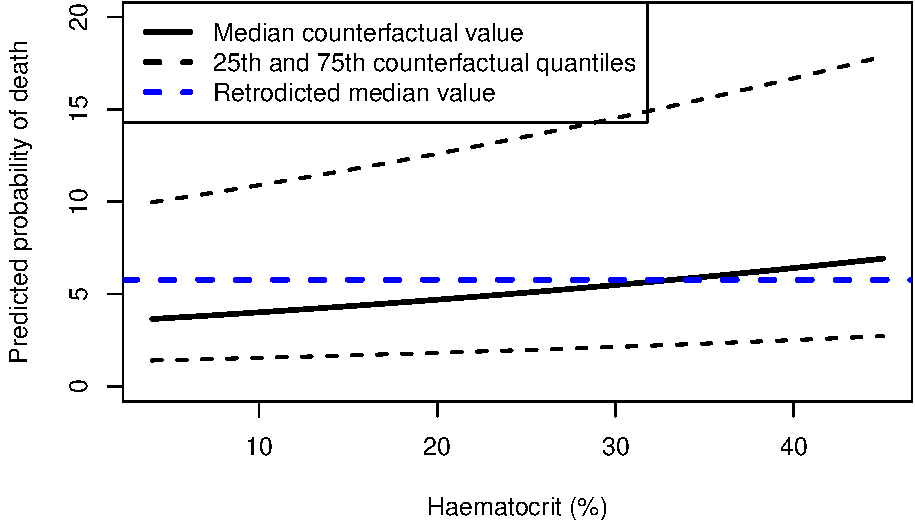
\includegraphics{LegacyAnalysis_files/figure-latex/unnamed-chunk-11-1.pdf}

\subsection{More complex GAM model}\label{more-complex-gam-model}

The GAM model allows for non-linear relationships between certain
variables and the outcome.

Here we fit as non-linear the effect of age and haematocrit on
mortality. We add a random effect term for the studyID We should also be
doing this for the study site\ldots{}

\begin{Shaded}
\begin{Highlighting}[]
\NormalTok{mod_full_GAM =}\StringTok{ }\KeywordTok{gam}\NormalTok{(outcome }\OperatorTok{~}\StringTok{ }\KeywordTok{s}\NormalTok{(HCT,AgeInYear) }\OperatorTok{+}\StringTok{ }\NormalTok{LPAR_pct  }\OperatorTok{+}\StringTok{ }\NormalTok{coma }\OperatorTok{+}\StringTok{ }\NormalTok{convulsions }\OperatorTok{+}
\StringTok{                     }\NormalTok{poedema }\OperatorTok{+}\StringTok{ }\KeywordTok{log10}\NormalTok{(BUN) }\OperatorTok{+}\StringTok{ }\NormalTok{BD }\OperatorTok{+}\StringTok{ }\NormalTok{drug_AS }\OperatorTok{+}\StringTok{ }
\StringTok{                     }\KeywordTok{s}\NormalTok{(studyID, }\DataTypeTok{bs=}\StringTok{'re'}\NormalTok{) }\OperatorTok{+}\StringTok{ }\KeywordTok{s}\NormalTok{(country, }\DataTypeTok{bs=}\StringTok{'re'}\NormalTok{),}
                   \DataTypeTok{data=}\NormalTok{Complete_Leg_data, }\DataTypeTok{family=}\NormalTok{binomial)}
\KeywordTok{summary}\NormalTok{(mod_full_GAM)}
\end{Highlighting}
\end{Shaded}

\begin{verbatim}
## 
## Family: binomial 
## Link function: logit 
## 
## Formula:
## outcome ~ s(HCT, AgeInYear) + LPAR_pct + coma + convulsions + 
##     poedema + log10(BUN) + BD + drug_AS + s(studyID, bs = "re") + 
##     s(country, bs = "re")
## 
## Parametric coefficients:
##               Estimate Std. Error z value Pr(>|z|)    
## (Intercept)  -6.327596   0.270364 -23.404  < 2e-16 ***
## LPAR_pct      0.001766   0.060455   0.029 0.976696    
## coma          1.330827   0.100888  13.191  < 2e-16 ***
## convulsions1  0.534704   0.117346   4.557  5.2e-06 ***
## poedema1      0.547871   0.384139   1.426 0.153801    
## log10(BUN)    1.701401   0.170552   9.976  < 2e-16 ***
## BD            0.123330   0.007331  16.824  < 2e-16 ***
## drug_AS      -0.343908   0.090360  -3.806 0.000141 ***
## ---
## Signif. codes:  0 '***' 0.001 '**' 0.01 '*' 0.05 '.' 0.1 ' ' 1
## 
## Approximate significance of smooth terms:
##                       edf Ref.df Chi.sq  p-value    
## s(HCT,AgeInYear) 5.487067  7.664 33.634 3.60e-05 ***
## s(studyID)       0.004292  5.000  0.003    0.496    
## s(country)       9.942725 14.000 74.592 2.79e-15 ***
## ---
## Signif. codes:  0 '***' 0.001 '**' 0.01 '*' 0.05 '.' 0.1 ' ' 1
## 
## R-sq.(adj) =   0.27   Deviance explained = 29.1%
## UBRE = -0.43785  Scale est. = 1         n = 6116
\end{verbatim}

Now we compute the corresponding counterfactual probabilities of death
for the dataset for all values of the haematocrit:

\begin{Shaded}
\begin{Highlighting}[]
\NormalTok{overall_median_mortalityGAM =}\StringTok{ }\KeywordTok{median}\NormalTok{(}\DecValTok{100}\OperatorTok{*}\KeywordTok{predict}\NormalTok{(mod_full_GAM, }\DataTypeTok{type=}\StringTok{'response'}\NormalTok{))}
\KeywordTok{par}\NormalTok{(}\DataTypeTok{las=}\DecValTok{1}\NormalTok{, }\DataTypeTok{bty=}\StringTok{'n'}\NormalTok{)}
\NormalTok{probs_gam =}\StringTok{ }\KeywordTok{array}\NormalTok{(}\DataTypeTok{dim =} \KeywordTok{c}\NormalTok{(}\DecValTok{3}\NormalTok{, }\KeywordTok{length}\NormalTok{(x_hcts)))}
\ControlFlowTok{for}\NormalTok{(i }\ControlFlowTok{in} \DecValTok{1}\OperatorTok{:}\KeywordTok{length}\NormalTok{(x_hcts))\{}
\NormalTok{  mydata =}\StringTok{ }\NormalTok{Complete_Leg_data}
\NormalTok{  mydata}\OperatorTok{$}\NormalTok{HCT=x_hcts[i]}
\NormalTok{  ys =}\StringTok{ }\DecValTok{100}\OperatorTok{*}\KeywordTok{predict}\NormalTok{(mod_full_GAM, }\DataTypeTok{newdata =}\NormalTok{ mydata, }\DataTypeTok{type=}\StringTok{'response'}\NormalTok{)}
\NormalTok{  probs_gam[,i] =}\StringTok{ }\KeywordTok{quantile}\NormalTok{(ys, }\DataTypeTok{probs=}\NormalTok{myquantiles)}
\NormalTok{\}}
\end{Highlighting}
\end{Shaded}

We see that the effect of haematocrit on mortality is non-linear under
this model: below 20 is protective, above 20 plateaus out:

\begin{Shaded}
\begin{Highlighting}[]
\CommentTok{#}
\KeywordTok{par}\NormalTok{(}\DataTypeTok{las=}\DecValTok{1}\NormalTok{, }\DataTypeTok{mfrow=}\KeywordTok{c}\NormalTok{(}\DecValTok{1}\NormalTok{,}\DecValTok{2}\NormalTok{), }\DataTypeTok{bty=}\StringTok{'n'}\NormalTok{, }\DataTypeTok{mar=}\KeywordTok{c}\NormalTok{(}\DecValTok{4}\NormalTok{,}\DecValTok{4}\NormalTok{,}\DecValTok{1}\NormalTok{,}\DecValTok{1}\NormalTok{))}
\NormalTok{### Plot the standard logistic regression model}
\KeywordTok{plot}\NormalTok{(x_hcts,probs_lin[}\DecValTok{2}\NormalTok{,], }\DataTypeTok{xlim=}\KeywordTok{c}\NormalTok{(}\DecValTok{4}\NormalTok{,}\DecValTok{45}\NormalTok{), }\DataTypeTok{ylab=}\StringTok{'Predicted probability of death'}\NormalTok{, }
     \DataTypeTok{xlab=}\StringTok{'Haematocrit (%)'}\NormalTok{, }\DataTypeTok{ylim=}\KeywordTok{c}\NormalTok{(}\DecValTok{0}\NormalTok{,}\DecValTok{20}\NormalTok{), }\DataTypeTok{lty=}\DecValTok{1}\NormalTok{, }\DataTypeTok{lwd=}\DecValTok{3}\NormalTok{, }\DataTypeTok{type=}\StringTok{'l'}\NormalTok{)}
\KeywordTok{lines}\NormalTok{(x_hcts, probs_lin[}\DecValTok{1}\NormalTok{,], }\DataTypeTok{lty=}\DecValTok{2}\NormalTok{, }\DataTypeTok{lwd=}\DecValTok{2}\NormalTok{)}
\KeywordTok{lines}\NormalTok{(x_hcts, probs_lin[}\DecValTok{3}\NormalTok{,], }\DataTypeTok{lty=}\DecValTok{2}\NormalTok{, }\DataTypeTok{lwd=}\DecValTok{2}\NormalTok{)}
\KeywordTok{abline}\NormalTok{(}\DataTypeTok{h=}\NormalTok{overall_median_mortality, }\DataTypeTok{lwd=}\DecValTok{3}\NormalTok{, }\DataTypeTok{col=}\StringTok{'blue'}\NormalTok{,}\DataTypeTok{lty=}\DecValTok{2}\NormalTok{)}
\KeywordTok{title}\NormalTok{(}\StringTok{'Logistic regression model'}\NormalTok{)}
\NormalTok{### And now the GAM model}
\KeywordTok{plot}\NormalTok{(x_hcts,probs_gam[}\DecValTok{2}\NormalTok{,], }\DataTypeTok{xlim=}\KeywordTok{c}\NormalTok{(}\DecValTok{4}\NormalTok{,}\DecValTok{45}\NormalTok{), }\DataTypeTok{ylab=}\StringTok{'Predicted probability of death'}\NormalTok{, }
     \DataTypeTok{xlab=}\StringTok{'Haematocrit (%)'}\NormalTok{, }\DataTypeTok{ylim=}\KeywordTok{c}\NormalTok{(}\DecValTok{0}\NormalTok{,}\DecValTok{20}\NormalTok{), }\DataTypeTok{lty=}\DecValTok{1}\NormalTok{, }\DataTypeTok{lwd=}\DecValTok{3}\NormalTok{, }\DataTypeTok{type=}\StringTok{'l'}\NormalTok{)}
\KeywordTok{lines}\NormalTok{(x_hcts, probs_gam[}\DecValTok{1}\NormalTok{,], }\DataTypeTok{lty=}\DecValTok{2}\NormalTok{, }\DataTypeTok{lwd=}\DecValTok{2}\NormalTok{)}
\KeywordTok{lines}\NormalTok{(x_hcts, probs_gam[}\DecValTok{3}\NormalTok{,], }\DataTypeTok{lty=}\DecValTok{2}\NormalTok{, }\DataTypeTok{lwd=}\DecValTok{2}\NormalTok{)}
\KeywordTok{abline}\NormalTok{(}\DataTypeTok{h=}\NormalTok{overall_median_mortalityGAM, }\DataTypeTok{lwd=}\DecValTok{3}\NormalTok{, }\DataTypeTok{col=}\StringTok{'blue'}\NormalTok{,}\DataTypeTok{lty=}\DecValTok{2}\NormalTok{)}
\KeywordTok{title}\NormalTok{(}\StringTok{'Generalised additive model'}\NormalTok{)}
\end{Highlighting}
\end{Shaded}

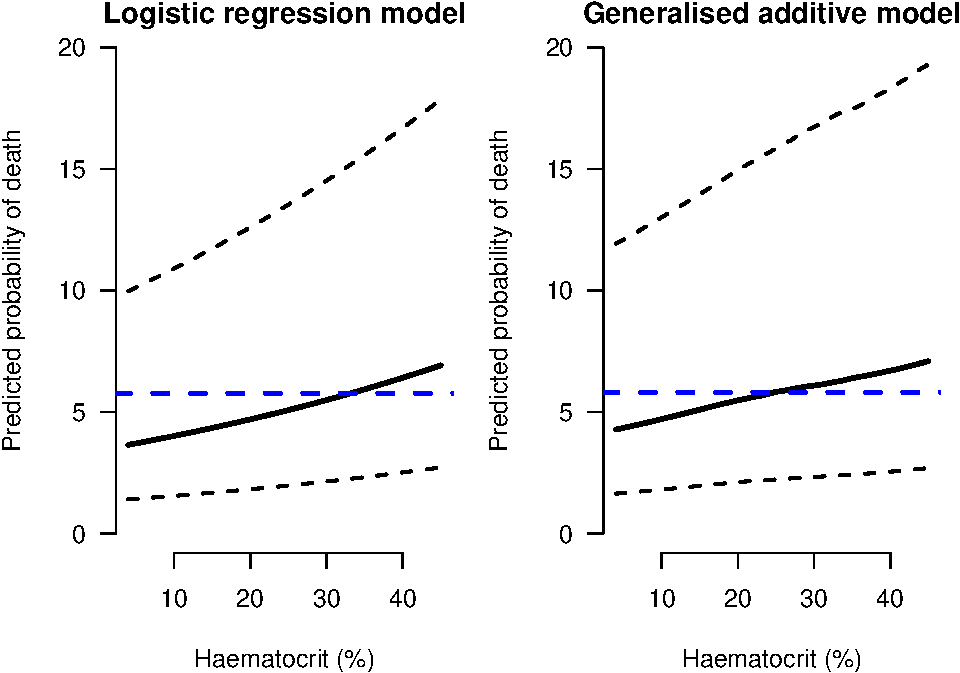
\includegraphics{LegacyAnalysis_files/figure-latex/counterfactualPlots-1.pdf}

\subsection{Model comparison}\label{model-comparison}

Which model is better fit in terms of AIC

\begin{Shaded}
\begin{Highlighting}[]
\KeywordTok{print}\NormalTok{(}\KeywordTok{AIC}\NormalTok{(mod_full_GAM, mod_full_GLM))}
\end{Highlighting}
\end{Shaded}

\begin{verbatim}
##                    df      AIC
## mod_full_GAM 23.43408 3438.101
## mod_full_GLM 12.00000 3459.687
\end{verbatim}

And in terms of deviance

\begin{Shaded}
\begin{Highlighting}[]
\KeywordTok{print}\NormalTok{(}\KeywordTok{list}\NormalTok{(}\DataTypeTok{mod_full_GLM =} \KeywordTok{deviance}\NormalTok{(mod_full_GLM), }\DataTypeTok{mod_full_GAM=}\KeywordTok{deviance}\NormalTok{(mod_full_GAM)))}
\end{Highlighting}
\end{Shaded}

\begin{verbatim}
## $mod_full_GLM
## [1] 3400.304
## 
## $mod_full_GAM
## [1] 3391.233
\end{verbatim}


\end{document}
